\documentclass{article}
\usepackage[T1]{fontenc}
\usepackage{mathpazo}
\usepackage{kpfonts}
\usepackage{graphicx}

\begin{document}

\begin{itemize}
\item Here's humanity, and all that we know:

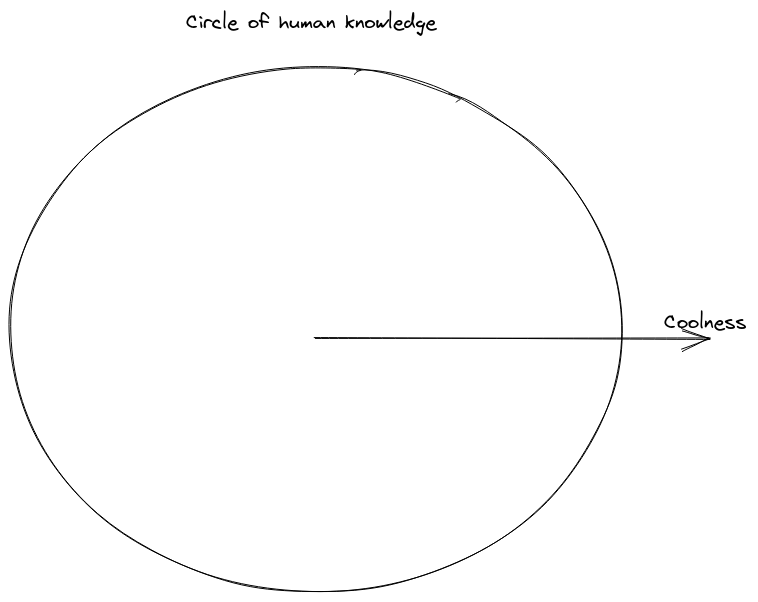
\includegraphics[width=0.8\textwidth]{./images/research-0.png}

\item Here's us beginning a new project, redoing what we already know. This is uninspired (gray),
  so we make sure to keep studying things we don't know (red)

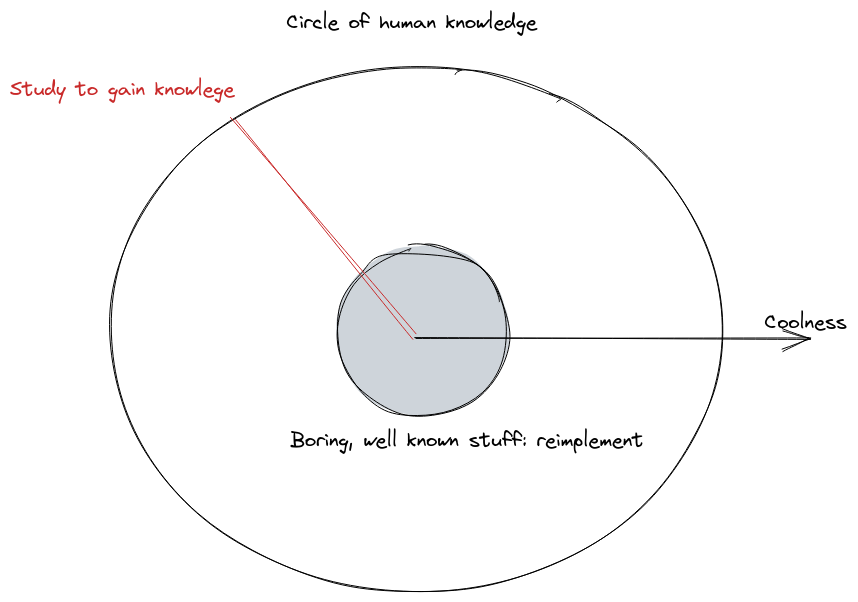
\includegraphics[width=0.8\textwidth]{./images/research-1.png}

\newpage

\item Here's us using what we learnt to extend the project. This is fun! We're applying what we learnt! See
  that our ball grows larger, misshapen. We continue studying new things though, that's one half of 
  what research is about.

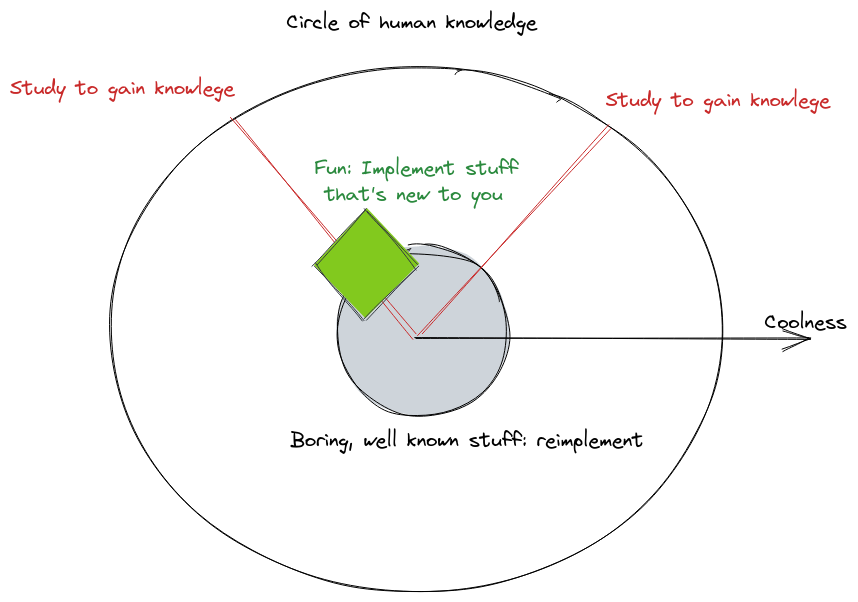
\includegraphics[width=0.8\textwidth]{./images/research-3.png}

\item Here's us repeating the strategy again. The weeks go by, as we study and accrue a bigger ball of fun, green mud
     that doesn't quite fit together:

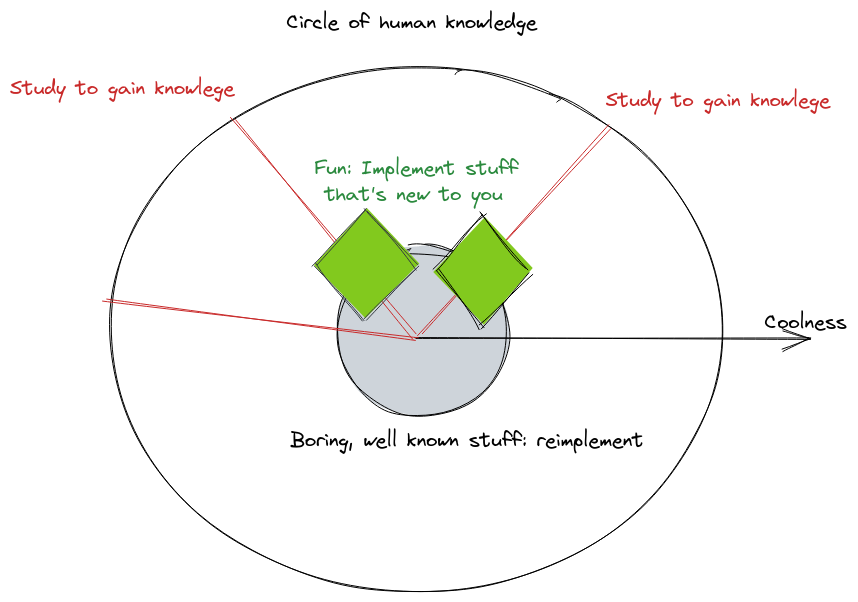
\includegraphics[width=0.8\textwidth]{./images/research-4.png}


\item After a few months, we have a respectable sized ball. It's odd, misshapen, has gotten much further along
  some directions than others. It's a ball we can now polish. Remember, pearls need grit to form around.

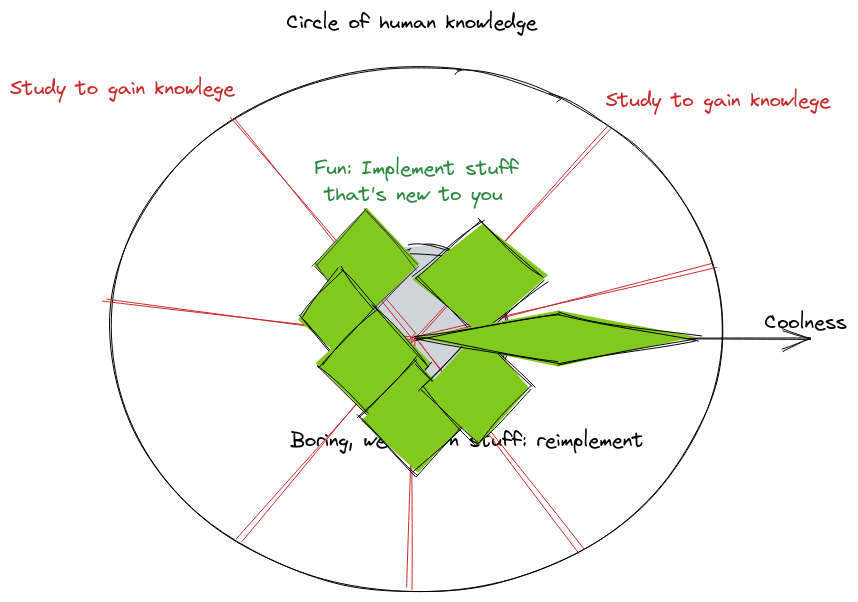
\includegraphics[width=0.8\textwidth]{./images/research-5.png}


\item From the large misshapen ball, we extract out a pearl (orange). It deeply
  develops one idea, that pushes human knowledge. It's smaller in many directions, since
  we've \emph{extracted} out the core insight. But it is indeed respectable, and fun, and the second
  half of research.

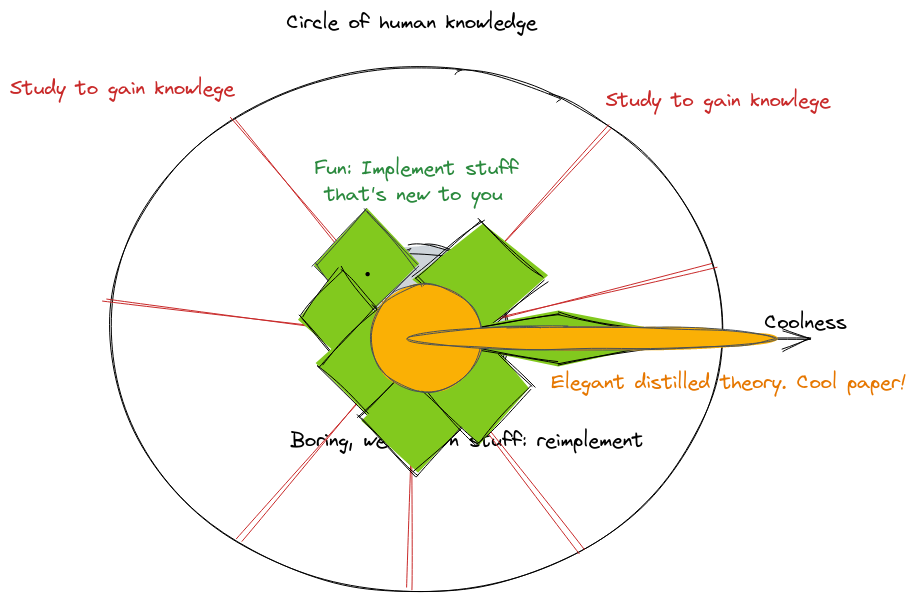
\includegraphics[width=0.8\textwidth]{./images/research-6.png}

\item We now have a larger ball, and a nice insight in one direction. We repeat the process, with the yellows and greens becoming gray,
  since we understand it well enough that it's now mundane. Onto the next greens to make the ball larger, misshapen, and fun!

\end{itemize}

\end{document}

